\setcounter{section}{0}

\section{Lecture 1: Introduction, Degrees of Freedom, and Lagrangian Dynamics}

\subsection{Introduction}

The objective of this course is to develop a deep understanding of classical dynamical systems using the framework of Lagrangian mechanics. This formulation elegantly generalizes Newtonian mechanics and provides powerful methods for dealing with complex, constrained systems.

\subsubsection*{Overview of Coordinate Systems}

The description of a physical system can vary significantly with the choice of coordinate system. Below are some common coordinate representations:

\paragraph{Cartesian Coordinates.}  
For a particle in three-dimensional space, the position, velocity, and acceleration are expressed as:
\begin{equation}
    \begin{aligned}
        \mathbf{r} &= (x,\, y,\, z), \\
        \mathbf{v} &= \dot{\mathbf{r}}, \\
        \mathbf{a} &= \ddot{\mathbf{r}}.
    \end{aligned}
\end{equation}

\paragraph{Polar Coordinates.}  
For planar motion, using polar coordinates $(r,\theta)$:
\begin{equation}
    \begin{aligned}
        \frac{d\hat{\mathbf{e}}_r}{dt} &= \dot{\theta}\,\hat{\mathbf{e}}_\theta, \\
        \frac{d\hat{\mathbf{e}}_\theta}{dt} &= -\dot{\theta}\,\hat{\mathbf{e}}_r,
    \end{aligned}
\end{equation}
so that the position and velocity become:
\begin{equation}
    \begin{aligned}
        \mathbf{r} &= r\,\hat{\mathbf{e}}_r, \\
        \mathbf{v} &= \dot{r}\,\hat{\mathbf{e}}_r + r\,\dot{\theta}\,\hat{\mathbf{e}}_\theta.
    \end{aligned}
\end{equation}

\paragraph{Spherical Coordinates.}  
For a particle in three-dimensional space described by spherical coordinates $(r, \theta, \phi)$:
\begin{equation}
    \begin{aligned}
        \mathbf{r} &= (r,\, \theta,\, \phi), \\
        \mathbf{v} &= \dot{r}\,\hat{\mathbf{r}} + r\,\dot{\theta}\,\hat{\boldsymbol{\theta}} + r\,\dot{\phi}\,\sin\theta\,\hat{\boldsymbol{\phi}}.
    \end{aligned}
\end{equation}

\subsection{Degrees of Freedom and Generalized Coordinates}

In classical mechanics, the \emph{degrees of freedom} (DOF) represent the number of independent parameters required to specify the configuration of a system.

\begin{definition}[Degrees of Freedom]
    \textbf{Mechanic definition:} The number of independent parameters needed to define a system's configuration.\\[1mm]
    \textbf{Kinetic definition:} For a rigid body, the DOF equals the number of independent movements (typically 3 translational and 3 rotational in three dimensions).
\end{definition}

For a system of \(M\) particles in three-dimensional space with no constraints, the total degrees of freedom is \(3M\). When \(N\) holonomic (i.e., integrable) constraints are present, the number of independent generalized coordinates reduces to:
\begin{equation}
    \text{DOF} = 3M - N.
\end{equation}

If there are additional \(k\) nonholonomic (non-integrable) constraints, these restrict the allowable velocities but do not reduce the configuration space's dimension. Thus, under the kinetic viewpoint, the effective degrees of freedom become:
\begin{equation}
    \text{DOF}_{\text{kinetic}} = 3M - N - k.
\end{equation}
Nevertheless, the number of generalized coordinates remains \(3M - N\).

\subsubsection*{Examples of Constrained Systems}

\begin{itemize}
    \item \textbf{Two particles connected by a rod:}\\[1mm]
          The rod fixes the distance between the particles, leading to:
          \begin{equation}
              \text{DOF} = 3\times2 - 1 = 5.
          \end{equation}

    \item \textbf{Four particles connected by rods with fixed angles:}\\[1mm]
          With three constraints fixing the rod lengths and three additional constraints fixing the angles, the system behaves as a rigid body:
          \begin{equation}
              \text{DOF} = 3\times4 - 3 \,(\text{length constraints}) - 3 \,(\text{angular constraints}) = 6.
          \end{equation}

    \item \textbf{Three particles connected by rods with one unfixed angle:}\\[1mm]
          Removing one angular constraint results in:
          \begin{equation}
              \text{DOF} = 3\times3 - 2 = 7.
          \end{equation}
\end{itemize}

\begin{figure}[ht]
    \centering
    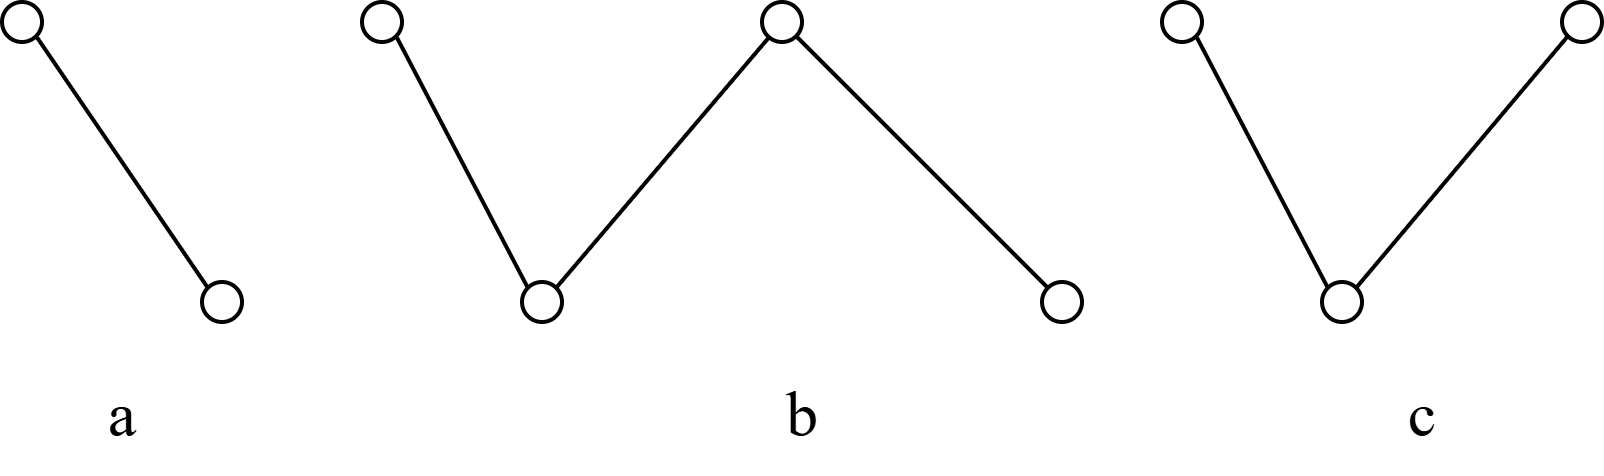
\includegraphics[width=0.8\textwidth]{images/1-1-1.png}
    \caption{Examples of Constrained Systems}
    \label{fig:1-1-1}
\end{figure}

\subsubsection*{The Simple Pendulum}

Consider the simple pendulum (see Figure~\ref{fig:1-1-2}). The motion of the pendulum is completely described by the angular displacement \(\theta\), thus it has one degree of freedom.

\begin{figure}[ht]
    \centering
    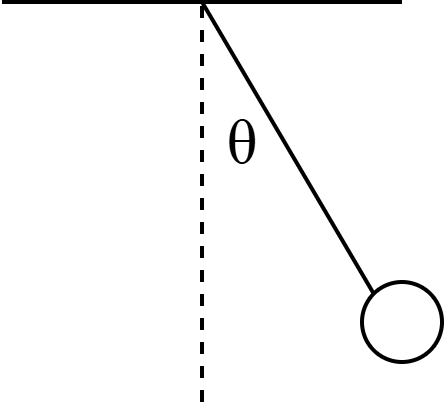
\includegraphics[width=0.3\textwidth]{images/1-1-2.png}
    \caption{Simple Pendulum}
    \label{fig:1-1-2}
\end{figure}

\subsubsection*{Generalized Coordinates in Constrained Systems}

For systems with constraints, we introduce generalized coordinates \(\{q_i\}\) (with \(i = 1, 2, \dots, N\)) such that the position of each particle \(\alpha\) is expressed as:
\begin{equation}
    \mathbf{r}_\alpha = \mathbf{r}_\alpha(q_1, q_2, \dots, q_N, t).
\end{equation}
When constraints explicitly depend on time, they are termed \emph{rheonomous}; otherwise, they are \emph{scleronomous}. Moreover, if a constraint can be written as
\[
f(q_1, q_2, \dots, q_N, t) = 0,
\]
(i.e., it does not involve velocities), it is a \emph{holonomic} constraint; constraints involving velocities are classified as \emph{nonholonomic}.

Nonholonomic systems frequently occur in practice. For example, consider a box moving on the surface of a sphere in figure \ref{fig:1-1-3}: when the box loses contact with the surface, the effective degrees of freedom increase.

\begin{figure}[ht]
    \centering
    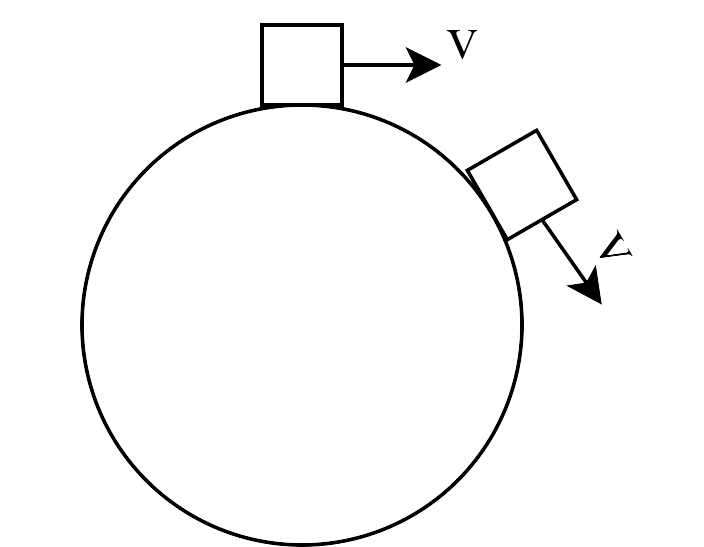
\includegraphics[width=0.3\textwidth]{images/1-1-3.png}
    \caption{Example of a Nonholonomic System}
    \label{fig:1-1-3}
\end{figure}

\subsection{Lagrangian Mechanics}

Lagrangian mechanics reformulates the equations of motion for a system in terms of generalized coordinates. Consider a system described by generalized coordinates \(q_i\) (\(i=1,2,\dots,N\)); the positions of its constituent particles can be expressed as:
\begin{equation}
    \mathbf{r}_\alpha = \mathbf{r}_\alpha(q_i, t).
\end{equation}
The primary task is to determine the evolution of \(q_i(t)\), governed by a set of \(N\) differential equations, known as the \emph{Euler-Lagrange equations}.

\subsubsection*{From Newton to Lagrange}

In the traditional Newtonian approach, one must:
\begin{enumerate}
    \item Compute the forces \(\mathbf{F}_\alpha\) acting on each particle.
    \item Apply Newton's second law:
          \begin{equation}
              \mathbf{F}_\alpha = m_\alpha \ddot{\mathbf{r}}_\alpha,
          \end{equation}
          yielding a set of second-order differential equations.
    \item Express \(\mathbf{r}_\alpha\) in terms of the generalized coordinates \(q_i\).
\end{enumerate}
This process can become cumbersome, particularly for systems with constraints.

\subsubsection*{Generalized Forces and Virtual Work}

Consider an infinitesimal virtual displacement \(\delta \mathbf{r}_\alpha\) of the particle positions, while time is held fixed. The corresponding virtual work done by the forces is given by:
\begin{equation}
    \delta W = \sum_\alpha \mathbf{F}_\alpha \cdot \delta \mathbf{r}_\alpha.
\end{equation}
Since the particle positions depend on the generalized coordinates, a variation in \(q_i\) induces:
\begin{equation} \label{eq:virtual_disp}
    \delta \mathbf{r}_\alpha = \sum_{i} \frac{\partial \mathbf{r}_\alpha}{\partial q_i}\delta q_i.
\end{equation}
Substituting into the virtual work expression,
\begin{equation}
    \delta W = \sum_{i} \left(\sum_\alpha \mathbf{F}_\alpha \cdot \frac{\partial \mathbf{r}_\alpha}{\partial q_i}\right)\delta q_i,
\end{equation}
we define the \emph{generalized force} \(Q_i\) as:
\begin{equation}
    Q_i = \sum_\alpha \mathbf{F}_\alpha \cdot \frac{\partial \mathbf{r}_\alpha}{\partial q_i}.
\end{equation}

\subsubsection*{Kinetic Energy and its Variations}

The kinetic energy of a system is
\begin{equation}
    T = \frac{1}{2}\sum_\alpha m_\alpha \dot{\mathbf{r}}_\alpha \cdot \dot{\mathbf{r}}_\alpha,
\end{equation}
which can be expressed as a function of the generalized coordinates and their time derivatives, \(T(q_i,\dot{q}_i,t)\). Since
\begin{equation}
    \dot{\mathbf{r}}_\alpha = \sum_i \frac{\partial \mathbf{r}_\alpha}{\partial q_i}\dot{q}_i + \frac{\partial \mathbf{r}_\alpha}{\partial t},
\end{equation}
it follows that
\begin{equation}
    \frac{\partial \dot{\mathbf{r}}_\alpha}{\partial \dot{q}_i} = \frac{\partial \mathbf{r}_\alpha}{\partial q_i}.
\end{equation}
Thus, the partial derivative of the kinetic energy with respect to \(q_i\) and \(\dot{q}_i\) is:
\begin{equation}
    \frac {\partial T}{\partial q_i}  = \sum_\alpha m_\alpha \dot{\mathbf{r}}_\alpha \cdot \frac{\partial \dot{\mathbf{r}}_\alpha}{\partial q_i}
\end{equation}
\begin{equation}
    \frac{\partial T}{\partial \dot{q}_i} = \sum_\alpha m_\alpha \dot{\mathbf{r}}_\alpha \cdot \frac{\partial \mathbf{r}_\alpha}{\partial q_i}.
\end{equation}
Taking the time derivative and using Newton's second law:
\begin{align}
    \frac{d}{dt} \left(\frac {\partial T}{\partial \dot{q_i}}\right) & = \sum_\alpha m_\alpha \left(\ddot{\mathbf{r}}_\alpha \cdot \frac{\partial \mathbf{r}_\alpha}{\partial q_i} + \dot{\mathbf{r}}_\alpha \cdot \frac{\partial \dot{\mathbf{r}}_\alpha}{\partial q_i}\right) \\
                                                                     & = \sum_\alpha \mathbf{F}_\alpha \cdot \frac{\partial \mathbf{r}_\alpha}{\partial q_i} + \frac{\partial T}{\partial q_i} \\
                                                                     & = Q_i + \frac{\partial T}{\partial q_i}  
\end{align}
One obtains the important relation:
\begin{equation}
    Q_i = \frac{d}{dt}\left(\frac{\partial T}{\partial \dot{q}_i}\right) - \frac{\partial T}{\partial q_i}.
\end{equation}
This result forms the foundation for deriving the Euler-Lagrange equations, which succinctly encapsulate the dynamics of the system.

\subsection{The Principle of Virtual Work and d'Alembert's Principle}

\subsubsection*{Principle of Virtual Work}

\paragraph{Applied Forces.}  These are the external forces actively acting on the system. They can include gravity, friction (if it does work), external loads, etc. Applied forces are usually responsible for driving the motion or deformation of the system.

\paragraph{Constraint Forces.}  These forces arise from the constraints imposed on the system—such as rods, surfaces, or other geometric restrictions—that limit the motion of the system's parts. A key aspect of ideal constraints is that the constraint forces do no work during any \emph{virtual displacement}.

The \emph{principle of virtual work} states that for a system in equilibrium, the total virtual work done by the applied forces during any virtual displacement (consistent with the constraints) is zero:
\begin{equation}
    \delta W = \sum_\alpha \mathbf{F}_\alpha \cdot \delta \mathbf{r}_\alpha = 0.
\end{equation}

\subsubsection*{d'Alembert's Principle}

d'Alembert's principle extends the principle of virtual work to dynamics. It introduces the concept of \emph{inertial forces} (or \emph{d'Alembert forces}) to reformulate Newton's second law into a form that is analogous to static equilibrium:
\begin{equation}
    \sum_\alpha \left( \mathbf{F}_\alpha - m_\alpha \ddot{\mathbf{r}}_\alpha \right) \cdot \delta \mathbf{r}_\alpha = 0.
\end{equation}

Here, the term \( -m_\alpha \ddot{\mathbf{r}}_\alpha \) can be interpreted as an inertial force. By including these forces, the dynamic problem is converted into a statics-like problem where the total virtual work (including contributions from both applied and inertial forces) vanishes.

